\documentclass[class=article , crop=false, titlepage, twoside, multi={itemize, figure, verbatim}, float=false]{standalone}

\usepackage{import} % Required for importing other .tex docs.  (import uses everything bw Begin and End Doc)
\usepackage{float} % Required for specifying the exact location of a figure or table
\usepackage{graphicx} % Required for including images
\usepackage{wrapfig}
\usepackage[pdftex,breaklinks,colorlinks=true,linkcolor=black,citecolor=blue,urlcolor=red,linktocpage=false,pagebackref=true,filecolor=magenta]{hyperref}%http://www.tug.org/applications/hyperref/manual.html#x1-100003.6
\usepackage{cite}
\usepackage[toc,title,page]{appendix}
\usepackage{pdfpages} % enables loading a pdf into the doc
\usepackage{makeidx}
\usepackage{glossaries} % must be after hyperref
\usepackage{blindtext}
\usepackage{enumitem}
%\usepackage{caption}

%\setlist[description]{leftmargin=\parindent,labelindent=\parindent}

%\renewcommand*{\bibname}{References} % renames the bibliography

\newcommand{\HRule}{\rule{\linewidth}{0.5mm}} % Command to make the lines in the title page

\graphicspath{{img/}{GIS_ChampionSection/img/}{awardsChapter/GIS_ChampionSection/img/}{brandPart/awardsChapter/GIS_ChampionSection/img/}{img/}{pairedProgSection/img/}{methodChapter/pairedProgSection/img/}{methodPart/methodChapter/pairedProgSection/img/}{documentationSection/img/}{methodChapter/documentationSection/img/}{methodPart/methodChapter/documentationSection/img/}{docStorageOrgSection/img/}{methodChapter/docStorageOrgSection/img/}{methodPart/methodChapter/docStorageOrgSection/img/}{QGisSection/img/}{toolsChapter/QGisSection/img/}{servicePart/toolsChapter/QGisSection/img/}{ESRISection/img/}{toolChapter/ESRISection/img/}{servicePart/toolChapter/ESRISection/img/}{../../../../source/}{../../source/}{servicePart/applicationsChapter/treasurerSection/img/}}

%\setlength\parindent{0pt} % eliminates indents


\def\titlename{Control Point}

\title{\HRule % Horizontal Line added
\\[.4cm] % space
\begin{figure}[H] % included image
\begin{center}	% centered horizontally

\includegraphics[scale=.45]{GIS_Logo_better.jpg}
\end{center}
\end{figure}
\Huge \bfseries \titlename \\ % Title text
\HRule \\[.4cm] % Horizontal Line added
\author{\Large Allegan County GIS \\\Large www.allegancounty.org/gis} % defines author
}  % inputs common title
\setcounter{tocdepth}{5}  % subparagraph and down
\begin{document}% document begins

\ifstandalone
%\frontmatter % turns off chapter numbering and uses roman numerals for page numbers
\maketitle % creates title page and blank page after title page
\tableofcontents % creates TOC and blank page
\clearpage
%\mainmatter % turns on chapter numbering, resets page numbering and uses arabic numerals for page numbers
\fi

\subsection{Control Points}
\medskip
\subsubsection[Editing Control Points]{Maintaining Cadastral Control Points}
\vspace{.1in}

\paragraph[Fabric Point Move to Feature Addin]{\textbf{ Install the Fabric Point Move to Feature Addin}}
\vspace{.1in}

{\Large $\Rightarrow$ Push the Configure Button}

\begin{figure}[h!]
\centering
    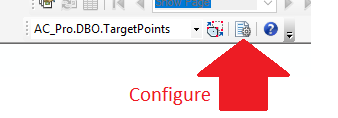
\includegraphics[width=.6\textwidth]{fabricPointMoveToFeatureAddIn.png}

\caption{Fabric Point Move to Feature Addin}
\end{figure}
%
\clearpage
  %
\paragraph[Configure Addin]{}\textbf{\Large Configure Addin}
\vspace{.1in}

\begin{itemize}

\item Set Reference Feature Layer to TargetPoints
\item Use point to point matching
\item Use point layer field: PointID
\end{itemize}

\begin{figure}[h!]
\centering
    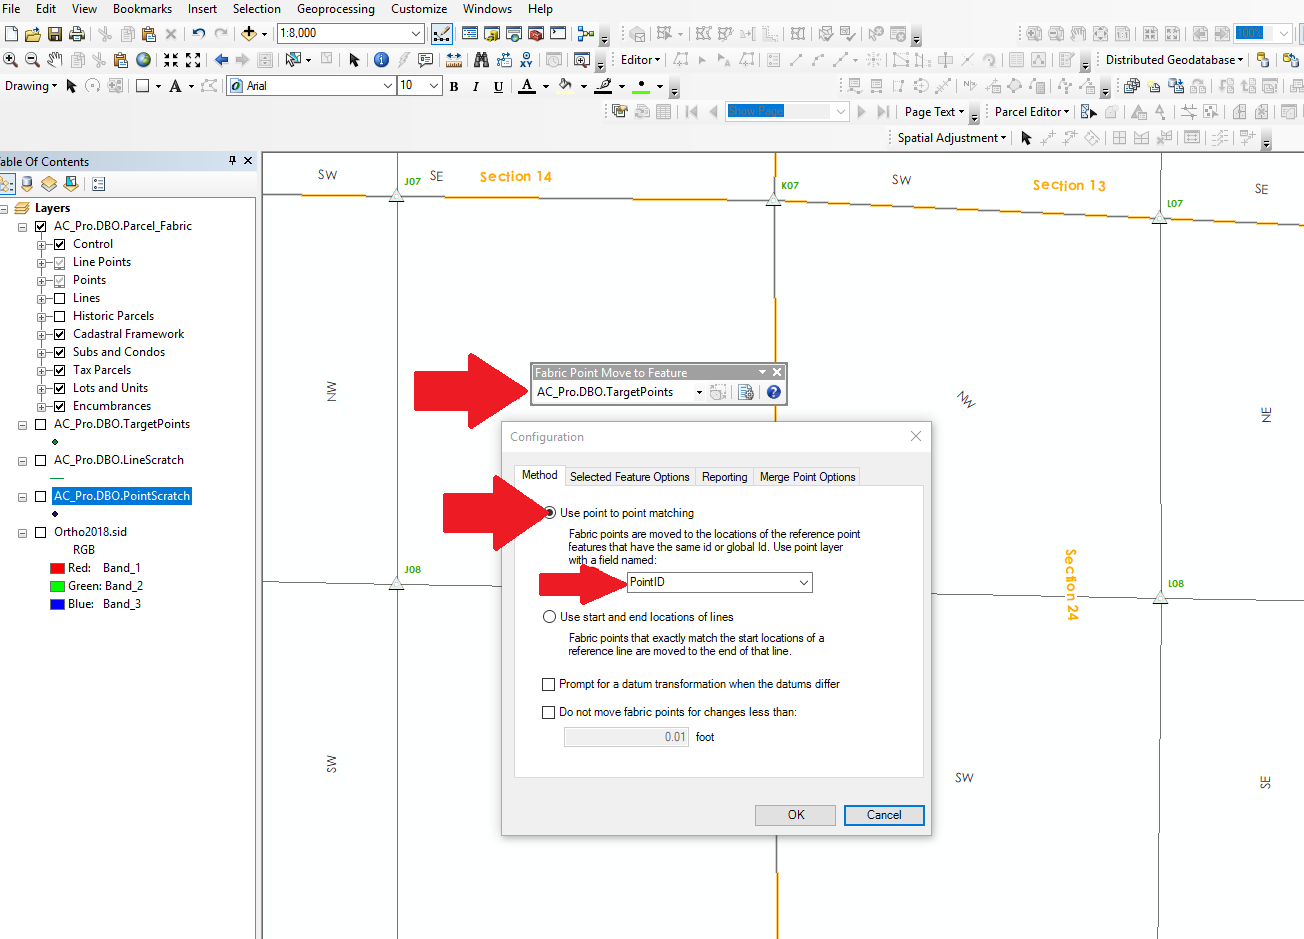
\includegraphics[width=.75\textwidth]{FabricPointMoveToFeatureConfigMethod.png}
\caption{Addin Configuration Method}
\end{figure}
%
%
\clearpage
%
%
%


\begin{verbatim}


  2
  Configure Fabric Point Move to Feature addin Selected Feature Options
  Move Fabric Points of the Selected Parcels
  Push OK
  FabricPointMoveToFeatureConfigSelectedFeatures.png

  3
  Identify position of new control point
  Select TargetPoints in Create Features Templates
  Create Target Point at location for new Control Point
  createTargetPoint.png

  4
  Use Identify tool to find ObjectID of Control Point that is to be moved
  Select the Target point PointID of the point its moving to
  Edit Target Point pointID attribute to match associated fabric control point OID
  updateTargetPointPointID.png

  4.5
  Push move point button
  moveControlPoint.png

  5
  Open maintain control point tool
  Select control Point
  push edit button
  maintainControlPointTool.png

  6
  Use Identify Tool to View X and Y vals for the point
  copy x and y value from point(attribute window) to Control (maintain control tool)
  push update
  Save Edits
  transferCoordinates.png




Identify position of new control point
Place Taarget Point
Update Target Point attributes to associated fabric point OID
Push move point button
Zoom to Control point
Open maintain control point tool
Select control Point
edit button
copy x and y value from
identify tool x and y of points
update button

\end{verbatim}
\end{document}
